%                      Code_Saturne version 1.3
%                      ------------------------
%
%     This file is part of the Code_Saturne Kernel, element of the
%     Code_Saturne CFD tool.
%
%     Copyright (C) 1998-2008 EDF S.A., France
%
%     contact: saturne-support@edf.fr
%
%     The Code_Saturne Kernel is free software; you can redistribute it
%     and/or modify it under the terms of the GNU General Public License
%     as published by the Free Software Foundation; either version 2 of
%     the License, or (at your option) any later version.
%
%     The Code_Saturne Kernel is distributed in the hope that it will be
%     useful, but WITHOUT ANY WARRANTY; without even the implied warranty
%     of MERCHANTABILITY or FITNESS FOR A PARTICULAR PURPOSE.  See the
%     GNU General Public License for more details.
%
%     You should have received a copy of the GNU General Public License
%     along with the Code_Saturne Kernel; if not, write to the
%     Free Software Foundation, Inc.,
%     51 Franklin St, Fifth Floor,
%     Boston, MA  02110-1301  USA
%
%-----------------------------------------------------------------------
%

\programme{condli}

\vspace{1cm}
%%%%%%%%%%%%%%%%%%%%%%%%%%%%%%%%%%
%%%%%%%%%%%%%%%%%%%%%%%%%%%%%%%%%%
\section{Fonction}
%%%%%%%%%%%%%%%%%%%%%%%%%%%%%%%%%%
%%%%%%%%%%%%%%%%%%%%%%%%%%%%%%%%%%
Il est n\'ecessaire de disposer de conditions aux limites dans au moins
trois cas principaux~:
\begin{itemize}
\item calcul de termes convectifs (diff\'erentiels d'ordre un en espace) au
bord~:  le calcul fait intervenir un flux au bord et demande
la donn\'ee au bord de la variable convect\'ee lorsque la fronti\`ere est
``entrante'' au sens des courbes caract\'eristiques du syst\`eme
(au sens de la vitesse, dans le cas d'une \'equation isol\'ee portant
sur un simple scalaire~: interpr\'etation suffisante dans le cadre actuel de
\CS\footnote{sauf en module compressible, cf. \fort{cfxtcl}})~;
\item calcul de termes de diffusion (diff\'erentiels d'ordre deux en espace)~:
il est alors n\'ecessaire de disposer d'un moyen de conna\^\i
tre la valeur
de d\'eriv\'ees spatiales d'ordre un au bord (plus exactement, il est
n\'ecessaire de disposer d'information permettant de calculer les termes qui en
d\'ependent, comme les contraintes ou les flux thermiques en paroi)~;
\item calcul de gradient ``cellules'' plus standard~: il est n\'ecessaire de disposer de la
donn\'ee de la variable aux faces de bord (plus g\'en\'eralement, il est n\'ecessaire
de disposer d'un moyen de calculer les termes discrets des \'equations
lorsqu'ils font intervenir le gradient dans les cellules de bord, comme par
exemple les termes de gradient transpos\'e des \'equations de Navier-Stokes).
\end{itemize}

Les consid\'erations pr\'esentes concernent uniquement les variables de calcul
(vitesse, pression, tenseur de Reynolds, scalaires solution d'une \'equation
de convection-diffusion). Pour ces grandeurs\footnote{
Les autres grandeurs
(propri\'et\'es physiques par
exemple) font l'objet d'un traitement diff\'erent qui ne sera pas d\'etaill\'e
ici (par exemple, pour la masse volumique, l'utilisateur d\'efinit directement
les valeurs aux bord, information qui est conserv\'ee telle quelle~; on pourra
se reportera \`a \fort{usphyv} ou \fort{phyvar}).
},
l'utilisateur doit d\'efinir
les conditions aux limites en chaque face de bord (\fort{usclim}).


Le sous-programme \fort{condli} permet de traduire les donn\'ees utilisateur
(fournies dans \fort{usclim}) au format interne de repr\'esentation des conditions
aux limites. Des v\'erifications de compl\'etude et de coh\'erence sont
\'egalement men\'ees (dans \fort{vericl}). Sont en particulier trait\'ees les conditions aux limites
de paroi (\fort{clptur})
et de sym\'etrie pour les vitesses et le tenseur de Reynolds (\fort{clsyvt}).

Le sous-programme \fort{condli} fournit en sortie des couples de coefficients
$A_b$ et $B_b$
pour chaque variable~$f$ et chaque face  de bord. Ils sont utilis\'es pour le calcul des
termes discr\'etis\'es intervenant dans les \'equations \`a r\'esoudre et
permettent en particulier de d\'eterminer une valeur de face
de bord $f_{b,int}$ (localis\'ee au ``centre'' de la face de bord,
barycentre de ses sommets) par la
relation $f_{b,int} = A_b+B_b\,f_{I'}$ o\`u $f_{I'}$ est la valeur de
la variable au point
$I'$, projet\'e du centre de la cellule jouxtant le bord sur la droite
normale \`a
la face de bord et passant par son centre
(voir la figure~\ref{Base_Condli_fig_flux_condli}).

\begin{figure}[h]
\centerline{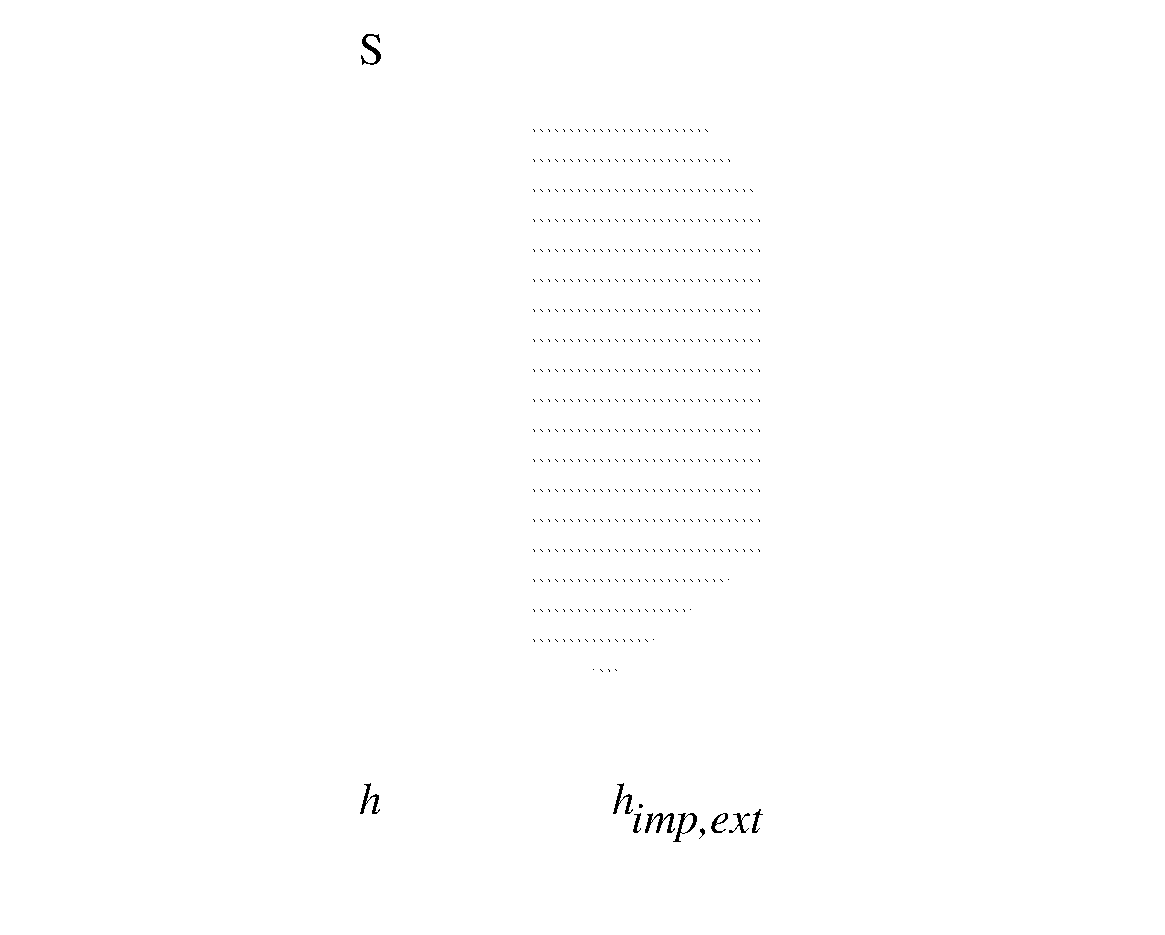
\includegraphics[height=8cm]{\repgraphics/fluxbord}}
\caption{\label{Base_Condli_fig_flux_condli}Cellule de bord.}
\end{figure}

%%%%%%%%%%%%%%%%%%%%%%%%%%%%%%%%%%
%%%%%%%%%%%%%%%%%%%%%%%%%%%%%%%%%%
\section{Discr\'etisation}
%%%%%%%%%%%%%%%%%%%%%%%%%%%%%%%%%%
%%%%%%%%%%%%%%%%%%%%%%%%%%%%%%%%%%

\etape{Notation}
%%%%%%%%%%%%%%%%
On d\'esignera dans la suite par {\it VarScalaire} toute variable
\begin{itemize}
\item [-] autre que la
vitesse, la pression, les grandeurs turbulentes $k$, $\varepsilon$,
$R_{ij}$, $\varphi$, $\bar{f}$ et $\omega$,
\item [-] solution d'une \'equation de convection-diffusion.
\end{itemize}
La d\'enomination {\it VarScalaire} pourra en particulier d\'esigner
la temp\'erature, un scalaire
passif, une fraction massique ou (sauf mention contraire explicite) la variance des fluctuations
d'une autre {\it VarScalaire}. Les variables d'\'etat d\'eduites (masse
volumique, viscosit\'e...) ne seront pas d\'esign\'ees par {\it VarScalaire}.


\etape{Repr\'esentation des conditions aux limites standard dans \fort{usclim} \vspace{0,3cm}}
%%%%%%%%%%%%%%%%%%%%%%%%%%%%%%%%%%%%%%%%%%%%%%%%%%%%%%%%%%%%%%%%%%%%%%%%%%%%%%%
Des conditions aux limites standardis\'ees peuvent \^etre fournies par
l'utilisateur dans \fort{usclim}. Il est pour cela n\'ecessaire d'affecter un
type aux
faces de bord des cellules concern\'ees\footnote{L'affectation d'un type se fait
en renseignant le tableau
\var{ITYPFB}.}. Les conditions pr\'evues par d\'efaut sont les suivantes~:



\begin{itemize}
\item [$\bullet$] {\bf Entr\'ee}~: correspond \`a une condition de Dirichlet sur
toutes les variables transport\'ees (vitesse, variables turbulentes,
{\it VarScalaires}...), et \`a
une condition de Neumann homog\`ene (flux nul) sur la pression.
\item [$\bullet$] {\bf Sortie}\label{Base_Condli_Sortie_Pression}~:
        \begin{itemize}
        \item [-] lorsque le flux de masse est effectivement dirig\'e vers
l'ext\'erieur du domaine, ce choix correspond \`a une condition de Neumann
homog\`ene sur toutes les variables transport\'ees et \`a
$\displaystyle\frac{\partial^2P}{\partial \vect{n}\partial\vect{\tau}_i}=0$, pris en compte sous forme
de Dirichlet pour la pression
($\vect{n}$ et $(\vect{\tau}_i)_{i \in \{1,2\}}$
d\'esignent respectivement le vecteur normal de la face de sortie consid\'er\'ee
et deux vecteurs norm\'es, orthogonaux entre eux et dans le plan de la face de
sortie). Cette condition est appliqu\'ee de
mani\`ere explicite en utilisant le champ de pression et son gradient
au pas de temps pr\'ec\'edent.
En outre, la pression \'etant d\'efinie \`a une
constante pr\`es, elle est recal\'ee en un point de
sortie pour y conserver la valeur \var{P0} (on \'evite ainsi toute d\'erive
vers des valeurs tr\`es grandes relativement \`a l'\'ecart maximal de
pression sur le domaine)\footnote{Lorsqu'il n'y a pas de sortie, le spectre des
valeurs propres de la matrice est d\'ecal\'e d'une valeur constante
afin de rendre le syst\`eme inversible~: voir \fort{matrix}.}.
        \item [-] lorsque le flux de masse est dirig\'e vers l'int\'erieur du
domaine, situation peu souhaitable {\it a priori}\footnote{Un message indique
\`a l'utilisateur combien de faces de sortie voient un flux de masse entrer dans
le domaine.
},
on impose une condition de
Dirichlet homog\`ene sur la vitesse (pas sur le flux de masse),
\`a d\'efaut de conna\^\i tre sa valeur en aval du domaine. La pression est
trait\'ee comme dans le cas pr\'ec\'edent o\`u le flux de masse est dirig\'e
vers l'ext\'erieur du domaine. Pour les variables
autres que la vitesse et la pression,
deux cas se pr\'esentent~:
                \begin{itemize}
                \item [-] dans le cas de sorties de type ``10''
(\var{ISOR10} dans \fort{usclim}), on
impose une condition de Dirichlet (valeur fournie par l'utilisateur et nulle par
d\'efaut) pour repr\'esenter la valeur du scalaire introduit dans le domaine
par les faces de bord concern\'ees.
                \item[-] dans le cas des sorties de type ``9''
(\var{ISOR09} dans \fort{usclim}), on
impose, comme lorsque le flux de masse est sortant, une condition de Neumann
homog\`ene (ceci n'est pas une situation souhaitable, puisque l'information
port\'ee sur les faces de bord provient alors de {\it l'aval} de l'\'ecoulement local).
                \end{itemize}
        \end{itemize}
\item [$\bullet$] {\bf Paroi}~: on se reportera \`a \fort{clptur} pour une description du
traitement des conditions aux limites de paroi (suppos\'ees imperm\'eables au
fluide). Bri\`evement, on peut dire ici
qu'une approche par lois de paroi est utilis\'ee afin d'imposer la contrainte
tangentielle sur la vitesse. La paroi peut \^etre d\'efilante\footnote{On doit alors fournir
les composantes de la vitesse de la paroi.}. Les {\it VarScalaires} re\c coivent par
d\'efaut une condition de Neumann homog\`ene (flux nul). Si l'on souhaite
imposer une valeur en paroi pour ces variables (par exemple, dans le cas d'une
paroi \`a temp\'erature impos\'ee)  une loi de similitude est utilis\'ee
pour d\'eterminer le flux au bord en tenant compte de la couche limite.
Dans le cas des couplages avec \syrthes, \CS
re\c coit une temp\'erature de paroi et fournit un flux thermique. La condition
de pression standard est une condition de Neumann homog\`ene\footnote{On pourra
se reporter \`a \fort{gradrc} pour la condition conduisant \`a l'extrapolation de
la pression au bord, condition pilotable par l'utilisation de la variable \var{EXTRAP}.}
\item [$\bullet$] {\bf Sym\'etrie}~: correspond \`a des conditions de Neumann homog\`enes pour les
grandeurs scalaires et \`a des conditions  de sym\'etrie classiques pour les vecteurs
(vitesse) et les tenseurs (tensions de Reynolds)~: voir \fort{clsyvt}.
\end{itemize}

\newpage

\etape{Repr\'esentation des conditions aux limites sp\'ecifiques dans \fort{usclim}\vspace{0,3cm}}
%%%%%%%%%%%%%%%%%%%%%%%%%%%%%%%%%%%%%%%%%%%%%%%%%%%%%%%%%%%%%%%%%%%%%%%%%%%%%%%
On a vu que l'affectation \`a une face de bord d'un type standard
(entr\'ee, sortie, paroi, sym\'etrie) permettait d'appliquer simplement
\`a l'ensemble des variables un assortiment de conditions aux limites
coh\'erentes entre elles pour les types usuels de fronti\`ere physique.

Une solution consiste \`a d\'efinir dans \fort{usclim},
pour chaque face de bord et chaque variable, des conditions aux limites
sp\'ecifiques\footnote{Les conditions
aux limites sp\'ecifiques sont cod\'ees en
renseignant directement les tableaux \var{ICODCL} et \var{RCODCL} pour chaque face de
bord et chaque variable~: des exemples sont fournis dans \fort{usclim}.}
(celles-ci, comme les conditions standards, se ram\`enent
finalement \`a des conditions de type mixte).

Les deux approches ne sont pas n\'ecessairement incompatibles et peuvent m\^eme
se r\'ev\'eler compl\'ementaires. En effet, les conditions aux limites standards
peuvent \^etre surcharg\'ees par l'utilisateur pour une ou plusieurs
variables donn\'ees. Il convient cependant de s'assurer que, d'une fa\c con ou
d'une autre, une condition \`a la limite a \'et\'e d\'efinie pour chaque face
de bord et chaque variable.

Des conditions de compatibilit\'e existent \'egalement entre les diff\'erentes
variables~(voir \fort{vericl}): \begin{itemize}
\item [-] en entr\'ee, paroi, sym\'etrie ou sortie libre, il est important que toutes les
composantes de la vitesse aient le m\^eme type de condition~;
\item [-] lorsque la vitesse re\c coit une condition de sortie, il est important
que la pression re\c coive une condition de type Dirichlet. Pour plus de
d\'etails, on se reportera au paragraphe relatif \`a la condition de sortie pour
la pression, page \pageref{Base_Condli_Sortie_Pression}~;
\item [-] lorsqu'une des variables de vitesse ou de turbulence
re\c coit une condition de paroi, il doit en \^etre de m\^eme pour toutes~;
\item [-] lorsqu'une des composantes $R_{ij}$ re\c coit une condition de sym\'etrie,
il doit en \^etre de m\^eme pour toutes~;
\item [-] lorsqu'une {\it VarScalaire} re\c coit une condition de paroi, la
vitesse doit avoir le m\^eme type de condition.
\end{itemize}

\newpage
\etape{Repr\'esentation interne des conditions aux limites}
%%%%%%%%%%%%%%%%%%%%%%%%%%%%%%%%%%%%%%%%%%%%%%%%%%%%%%%%%%%%%%%%%%%%%%%%%%%%%%%

{\bf Objectif}

Les conditions fournies par l'utilisateur sont
retraduites sous forme de couples de coefficients $A_b$ et $B_b$
pour chaque variable~$f$ et chaque face de bord. Ces coefficients
sont utilis\'es pour le calcul des
termes discrets intervenant dans les \'equations \`a r\'esoudre et
permettent en particulier de d\'eterminer une valeur de face
de bord $f_{b,int}$. Il est important d'insister d\`es \`a pr\'esent sur le fait
que cette valeur est, de mani\`ere g\'en\'erale, une simple valeur num\'erique
qui ne refl\`ete pas n\'ecessairement une r\'ealit\'e physique (en particulier
 aux parois, pour les grandeurs affect\'ees par la couche limite turbulente).
On d\'etaille ci-dessous le calcul de $A_b$, $B_b$ et de $f_{b,int}$.

{\bf Notations}
\begin{itemize}

\item[-] On consid\`ere l'\'equation (\ref{Base_Condli_eq_conv_diff_condli})
portant sur le scalaire $f$, dans laquelle
$\rho$ repr\'esente la masse volumique, $\vect{u}$ la vitesse, $\alpha$ la
conductivit\'e et
$S$ les termes sources additionnels. $C$ est d\'efini plus bas.
\begin{equation}\label{Base_Condli_eq_conv_diff_condli}
\displaystyle\rho\frac{\partial f}{\partial t} + div(\rho \vect{u} f)=div\left(\displaystyle\frac{\alpha}{C}\, \grad f\right)+S
\end{equation}

\item[-] Le coefficient $\alpha$ repr\'esente la somme des
conductivit\'es mol\'eculaire et turbulente (selon les mod\`eles utilis\'es), soit
$\alpha=\alpha_m+\alpha_t$, avec, pour une mod\'elisation de type viscosit\'e
turbulente, $\displaystyle\alpha_t=C\,\frac{\mu_t}{\sigma_t}$, o\`u $\sigma_t$ est le nombre de
Prandtl turbulent\footnote{Le nombre de Prandtl turbulent est sans dimension et,
dans certains cas usuels, pris \'egal \`a $0,7$.}.

\item[-] \`A titre d'exemple, on pr\'ecise dans le tableau \ref{Base_Condli_table_alpha_condli}
la valeur et l'unit\'e de $\alpha$ pour
quelques cas particuliers de $f$ (certains termes de l'\'equation peuvent alors
dispara\^\i tre~: pour la pression, en particulier, l'\'equation est
stationnaire et les termes convectifs sont absents).

\item[-] Le coefficient  $C_p$ repr\'esente la chaleur sp\'ecifique, d'unit\'e
                      $m^{2}\,s^{-2}\,K^{-1}=J\,kg^{-1}\,K^{-1}$.

\item[-] On note $\lambda$  la conductivit\'e thermique, d'unit\'e
$kg\,m\,s^{-3}\,K^{-1}=W\,m^{-1}\,K^{-1}$.

\item[-] Il convient de pr\'eciser que $C=1$ pour toutes les variables hormis
pour la temp\'erature, cas dans lequel on a\footnote{Plus exactement, on a
$C=C_p$ pour toutes les {\it VarScalaires} $f$ que l'on souhaite traiter comme la
temp\'erature pour les conditions aux limites. Ces {\it VarScalaires} sont
rep\'erables par l'utilisateur au moyen de l'indicateur \var{ISCSTH=1}. Par
d\'efaut cet indicateur est positionn\'e \`a la valeur 0 pour toutes les
{\it VarScalaires} (qui sont alors trait\'ees comme des scalaires passifs
avec $C=1$) hormis pour la variable
thermique \'eventuelle (\var{ISCALT}$^\text{i\`eme}$ {\it VarScalaire}), pour laquelle on a
\var{ISCSTH=1}~: on suppose par d\'efaut que la variable thermique est la temp\'erature et non
l'enthalpie. Si l'on souhaite r\'esoudre en enthalpie, il faut positionner
\var{ISCSTH} \`a la valeur 2 pour la variable thermique. Pour le compressible,
la variable thermique est l'�nergie, identifi�e par \var{ISCSTH=3}. On se
reportera � \fort{cfxtcl} pour le traitement des conditions aux limites.}
$C=C_p$. Dans le code, c'est la valeur de
$\displaystyle\frac{\alpha_m}{C}$ que l'utilisateur doit fournir (si la propri\'et\'e est
constante, les valeurs sont affect\'ees dans \fort{usini1} \`a \var{VISCL0} pour
la vitesse et \`a \var{VISLS0} pour les {\it VarScalaires}~; si la propri\'et\'e
est variable, ce sont des tableaux \'equivalents qui doivent \^etre renseign\'es
dans \fort{usphyv}).

\item[-] Pour la variance des fluctuations d'une {\it VarScalaire}, la
conductivit\'e $\alpha$ et le coefficient $C$ sont h\'erit\'es de la
{\it VarScalaire} associ\'ee.

\end{itemize}



\begin{table}
{\scriptsize
\begin{center}
\begin{tabular}{||l|l|l||l|l|l||}
\hline
\multicolumn{3}{||c||}{$f$}&\multicolumn{3}{|c||}{$\alpha$}\\
\hline
symbole              & nom                              & unit\'e                    &
symbole              & nom                              & unit\'e                  \\
\hline
$u_i$                & vitesse                          & $m\,s^{-1}$                &
$\mu$ ou $\mu+\mu_t$ & viscosit\'e dynamique            & $kg\,m^{-1}\,s^{-1}$     \\
$p$                  & pression                         & $kg\,m^{-1}\,s^{-2}$       &
$\Delta t$           & pas de temps                     & $s$                      \\
$T$                  & temp\'erature                    & $K$                        &
$\lambda$            & conductivit\'e thermique       & $kg\,m\,s^{-3}\,K^{-1}$ \\
                     &                                  &                            &
                     &                                  & $=W\,m^{-1}\,K^{-1}$\\
$H$                  & enthalpie                        & $m^{2}\,s^{-2}$&
$\lambda/C_p$        & conductivit\'e thermique/$C_p$ & $kg\,m^{-1}\,s^{-1}$     \\
                     &                                  & $=J\,kg^{-1}$&
                     &                                  &                          \\
$f$                  & {\it VarScalaire}                & unit\'e($f$)               &
$\alpha$             & conductivit\'e ou diffusivit\'e                   & $kg\,m^{-1}\,s^{-1}$     \\
\hline
\end{tabular}
\end{center}
}
\caption{Valeurs et unit\'es de $\alpha$ dans
quelques cas particuliers usuels.}\label{Base_Condli_table_alpha_condli}
\end{table}

%\newpage

{\bf Condition de type Dirichlet simple}~: lorsque la condition est une condition de Dirichlet simple, on
obtient naturellement (cas particulier de (\ref{Base_Condli_eq_fbord_condli}))~:
\begin{equation}
\underbrace{\ \ f_{b,int}\ \ }_{\text{valeur de bord utilis\'ee par le calcul}}
= \underbrace{\ \ f_{\text{\it r\'eel}}\ \ }_{\text{valeur r\'eelle impos\'ee au bord}}
\end{equation}
{\bf Autres cas}~: lorsque la condition \`a la limite porte
sur la donn\'ee d'un flux, il s'agit
d'un flux diffusif\footnote{En effet, le flux total sortant du domaine est
donn\'e par la
somme du flux convectif (si la variable est effectivement convect\'ee)
et du flux diffusif. N\'eanmoins, pour les parois
\'etanches et les sym\'etries, le flux de masse est nul et la condition se
r\'eduit \`a une contrainte sur le flux diffusif. De plus, pour les
sorties (flux de masse sortant), la condition \`a la limite ne porte que sur le
flux diffusif (souvent une condition de Neumann homog\`ene), le flux convectif
d\'ependant des conditions amont (il n'a donc pas besoin de
condition \`a la limite). Enfin, aux entr\'ees, c'est le plus souvent une
condition de Dirichlet simple qui est appliqu\'ee et le flux diffusif s'en d\'eduit.}.
On a alors~:
\begin{equation}
\underbrace{\ \ \phi_{int}\ \ }_{\text{flux diffusif transmis au domaine interne}}
= \underbrace{\ \ \phi_{\text{\it r\'eel}}\ \ }_{\text{flux diffusif r\'eel impos\'e au bord}}
\end{equation}

Le flux diffusif r\'eel impos\'e peut \^etre donn\'e
\begin{itemize}
\item [-] directement (condition de Neumann), soit
$\phi_{\text{\it r\'eel}}=\phi_{\text{\it imp,ext}}$ ou
\item [-] d\'eduit implicitement de deux informations impos\'ees~: une valeur
externe $f_{imp,ext}$ et un coefficient d'\'echange $h_{imp,ext}$
(condition de Dirichlet g\'en\'eralis\'ee).
\end{itemize}

\vspace{1cm}
Selon le type de condition (Dirichlet ou Neumann) et en prenant pour hypoth\`ese
la conservation du flux dans la direction normale au bord,
on peut alors \'ecrire (voir figure \ref{Base_Condli_fig_flux_condli})~:
\begin{equation}\label{Base_Condli_eq_flux_condli}
\begin{array}{l}
    \underbrace{h_{int}(f_{b,int}-f_{I'})}_{\phi_{int}}
  = \underbrace{h_{b}(f_{b,ext}-f_{I'})}_{\phi_{b}}
  = \left\{\begin{array}{ll}
    \underbrace{h_{imp,ext}(f_{imp,ext}-f_{b,ext})}_{\phi_{\text{\it r\'eel
impos\'e}}} &\text{(condition de Dirichlet)}\\
    \underbrace{\phi_{\text{\it imp,ext}}}_{\phi_{\text{\it r\'eel impos\'e}}}
            &\text{(condition de Neumann)}
           \end{array}\right.
\end{array}
\end{equation}

Le rapport entre le coefficient  $h_{b}$ et le coefficient $h_{int}$ rend compte
de l'importance de la travers\'ee de la zone proche du bord et
rev\^et une importance particuli\`ere dans le
cas des parois le long desquelles se d\'eveloppe une couche limite (dont les
propri\'et\'es sont alors prises en compte par $h_{b}$~: se reporter \`a
\fort{clptur}). Dans le cadre plus simple consid\'er\'e ici, on se limitera au
cas  $h_{b}=h_{int}$ et $f_{b,ext}=f_{b,int}=f_{b}$.
La relation (\ref{Base_Condli_eq_flux_condli}) s'\'ecrit alors~:

\begin{equation}
\underbrace{h_{int}(f_{b}-f_{I'})}_{\phi_{int}}
  = \left\{\begin{array}{ll}
    \underbrace{h_{imp,ext}(f_{imp,ext}-f_{b})}_{\phi_{\text{\it r\'eel
impos\'e}}} &\text{(condition de Dirichlet)}\\
    \underbrace{\phi_{\text{\it imp,ext}}}_{\phi_{\text{\it r\'eel impos\'e}}}
            &\text{(condition de Neumann)}
           \end{array}\right.
\end{equation}

En r\'earrangeant, on obtient la valeur de bord~:
\begin{equation}\label{Base_Condli_eq_fbord_condli}
f_{b}
  = \left\{\begin{array}{cccccl}
    \displaystyle\frac{h_{imp,ext}}{h_{int}+h_{imp,ext}}&f_{imp,ext}&+&
    \displaystyle\frac{h_{int}}{h_{int}+h_{imp,ext}}    &f_{I'}
                         &\text{(condition de Dirichlet)}\\
    \displaystyle\frac{1}{h_{int}}&\phi_{\text{\it imp,ext}}&+&
    \ &f_{I'}
            &\text{(condition de Neumann)}
           \end{array}\right.
\end{equation}


{\bf Conclusion}~: on notera donc les conditions aux limites
de mani\`ere g\'en\'erale sous la forme~:
\begin{equation}
f_{b}=A_b + B_b\,f_{I'}
\end{equation}
avec $A_b$ et $B_b$ d\'efinis selon le type des conditions~:
\begin{equation}
\begin{array}{c}
\text{Dirichlet}\left\{\begin{array}{ll}
    A_b = &\displaystyle\frac{h_{imp,ext}}{h_{int}+h_{imp,ext}}f_{imp,ext}\\
    B_b = &\displaystyle\frac{h_{int}}{h_{int}+h_{imp,ext}}
                  \end{array}\right.
\text{\ \  Neumann}\left\{\begin{array}{ll}
    A_b = &\displaystyle\frac{1}{h_{int}}\phi_{\text{\it imp,ext}}\\
    B_b = &1
                  \end{array}\right.
\end{array}
\end{equation}


\newpage

{\bf Remarques }
\begin{itemize}
\item [-] La valeur $f_{I'}$ est calcul\'ee en utilisant le gradient cellule de $f$,
soit~: $f_{I'}=f_{I}+\vect{II'}\grad{f}_I$.
\item [-] Il reste \`a pr\'eciser la valeur de $h_{int}$. Il s'agit d'une valeur {\it
num\'erique}, n'ayant {\it a priori} aucun rapport avec un coefficient d'\'echange
physique, et d\'ependante du mode de calcul du flux diffusif dans la premi\`ere
maille de bord. Ainsi~$\displaystyle h_{int}=\displaystyle\frac{\alpha}{\overline{I'F}}$
(l'unit\'e s'en d\'eduit naturellement).
\item [-] On rappelle que dans le code, c'est la valeur de
$\displaystyle\frac{\alpha_m}{C}$ que l'utilisateur doit fournir. Si la propri\'et\'e est
constante, les valeurs sont affect\'ees dans \fort{usini1} \`a \var{VISCL0} pour
la vitesse (viscosit\'e dynamique mol\'eculaire $\mu$ en $kg\,m^{-1}\,s^{-1}$)
et \`a \var{VISLS0} pour les {\it VarScalaires} (par exemple, pour la
temp\'erature et l'enthalpie, $\displaystyle\frac{\lambda}{C_p}$ en $kg\,m^{-1}\,s^{-1}$).
Si la propri\'et\'e est variable en espace ou en temps, ce sont des tableaux \'equivalents
qui doivent \^etre renseign\'es dans \fort{usphyv}.  En outre, la variance
des fluctuations d'une {\it VarScalaire} h\'erite automatiquement la valeur
de $\displaystyle\frac{\alpha_m}{C}$ de la {\it VarScalaire} associ\'ee
(\CS~1.1 et suivantes).
\item [-] On rappelle \'egalement, car ce peut \^etre source d'erreur, que dans
le code, on a~:
        \begin{itemize}
        \item [-] pour la temp\'erature $\alpha_m=\lambda$ et $C=C_p$
        \item [-] pour l'enthalpie      $\alpha_m=\displaystyle\frac{\lambda}{C_p}$ et $C=1$
        \end{itemize}
\end{itemize}


{\bf Exemples de cas particuliers}
\begin{itemize}
\item [-] Dans le cas d'une condition de Dirichlet,
l'utilisateur est donc conduit \`a
fournir deux donn\'ees :  $f_{imp,ext}$ et $h_{imp,ext}$.
Pour obtenir une condition de Dirichlet simple (sans coefficient d'\'echange)
il suffit d'imposer $h_{imp,ext}=+\infty$. C'est le cas d'utilisation le plus
courant (en pratique, $h_{imp,ext}=10^{30}$ ).
\item [-] Dans le cas d'une condition de Neumann, l'utilisateur fournit une seule valeur
$\phi_{\text{\it imp,ext}}$ (nulle pour les conditions de Neumann homog\`enes).
\end{itemize}


{\bf Valeur et unit\'e des donn\'ees \`a fournir}\\
Le tableau \ref{Base_Condli_table_h_phi_condli}
permet d'identifier les unit\'es de $h$ ($h_{imp,ext}$ ou
$h_{int}$) et $\phi_{\text{\it imp,ext}}$ pour quelques variables classiques. La
variable $d$ repr\'esente une longueur (\'egale, pour $h_{int}$, \`a
$\overline{I'F}$).
Il est \'egalement important de noter qu'un flux ``sortant'' doit \^etre positif.

\begin{table}
%{\tiny
\begin{center}
\begin{tabular}{||l|l|l||l|l||}
\hline
\multicolumn{3}{||c||}{$f$}&
\multicolumn{2}{c||}{$h$}     \\
\hline
symbole                         & nom                        & unit\'e         &
homog\`ene \`a                  & unit\'e                     \\
\hline
$u_i$                           & vitesse                    & $m\,s^{-1}$     &
$(\mu+\mu_t)/d$                 & $kg\,m^{-2}\,s^{-1}$       \\
$p$                             & pression                   & $kg\,m^{-1}\,s^{-2}$ &
$(\Delta t)/d$                  & $s\,m^{-1}$                \\
$T$                             & temp\'erature              & $K$         &
$(\lambda+C_p\mu_t/\sigma_t)/d$  &$kg\,s^{-3}\,K^{-1}$\\
                                &                            &                 &
                                & \ \                          $=W\,m^{-2}\,K^{-1}$\\
$H$                             & enthalpie                  & $m^{2}\,s^{-2}=J\,kg^{-1}$&
$(\lambda/C_p+\mu_t/\sigma_t)/d$ &$kg\,m^{-2}\,s^{-1}$\\
$f$                             & scalaire                   & unit\'e($f$)               &
$\alpha/d$                      & $kg\,m^{-2}\,s^{-1}$       \\
\hline
\end{tabular}
\end{center}
%}

%{\tiny
\begin{center}
\begin{tabular}{||l|l|l||l|l||}
\hline
\multicolumn{3}{||c||}{$f$}&
\multicolumn{2}{c||}{$\phi_{\text{\it imp,ext}}$} \\
\hline
symbole                         & nom                        & unit\'e         &
homog\`ene \`a                  & unit\'e                                     \\
\hline
$u_i$                           & vitesse                    & $m\,s^{-1}$     &
$(\mu+\mu_t)\,\grad{(\vect{u}_i)}.\vect{n}$  & $kg\,m^{-1}\,s^{-2} $                    \\
$p$                             & pression                   & $kg\,m^{-1}\,s^{-2}$ &
$(\Delta t)\,\grad{(p)}.\vect{n}$          & $kg\,m^{-2}\,s^{-1}$                        \\
$T$                             & temp\'erature              & $K$         &
$(\lambda+C_p\mu_t/\sigma_t)\,\grad{(T)}.\vect{n}$ &$kg\,s^{-3}=W\,m^{-2}$        \\
$H$                             & enthalpie                  & $m^{2}\,s^{-2}=J\,kg^{-1}$&
$(\lambda/C_p+\mu_t/\sigma_t)\,\grad{(H)}.\vect{n}$ &$kg\,s^{-3}=W\,m^{-2}$        \\
$f$                             & scalaire                   & unit\'e($f$)               &
$\alpha\,\grad{(f)}.\vect{n}$              & $kg\,m^{-2}\,s^{-1}$ unit\'e($f$)       \\
\hline
\end{tabular}
\end{center}
%}
\caption{Valeur et unit\'e de $h$ et $\phi_{\text{\it imp,ext}}$  dans
quelques cas particuliers usuels.}\label{Base_Condli_table_h_phi_condli}
\end{table}

\newpage
\etape{Condition de sortie pour la pression\vspace{0,3cm}}
%%%%%%%%%%%%%%%%%%%%%%%%%%%%%%%%%%%%%%%%%%%%%%%%%%%%%%%%%%%%%%%%%%%%
On pr\'ecise ici la condition de sortie appliqu\'ee
\`a la pression dans le cas des sorties standards.
Il est n\'ecessaire d'imposer une condition de type Dirichlet (accompagn\'ee d'une
condition
de type Neumann homog\`ene sur les composantes de la vitesse). On la
calcule \`a partir des valeurs de la variable au pas de temps pr\'ec\'edent.
\begin{itemize}
\item [-] En raisonnant sur une configuration simple (de type canal, avec une sortie
plane, perpendiculaire \`a l'\'ecoulement),
on peut faire l'hypoth\`ese que la forme des profils de pression pris
sur les surfaces parall\`eles \`a la sortie est inchang\'ee aux alentours de
celle-ci (hypoth\`ese d'un \'ecoulement \'etabli, loin de toute
perturbation). Dans cette situation, on peut \'ecrire
$\displaystyle\frac{\partial^2P}{\partial\vect{n}\partial\vect{\tau}_i}=0$
($\vect{n}$ est le vecteur normal \`a la sortie, $\vect{\tau}_i$ repr\'esente
une base du plan de sortie).

\item [-] Si, de plus,
on peut supposer que le gradient de pression pris dans la direction
perpendiculaire aux faces de sortie est uniforme au
voisinage de celle-ci, le profil \`a imposer en sortie (valeurs $p_b$)
se d\'eduit du profil
pris sur un plan amont (valeurs $p_{amont}$) en ajoutant simplement la constante
$R=d\,\grad{(p)}.\vect{n}$ (o\`u $d$ est la distance entre le plan amont
et la sortie), soit $p_b=p_{amont}+R$ (le fait que $R$ soit identique pour
toutes les faces de sortie est important afin de pouvoir l'\'eliminer dans
l'\'equation (\ref{Base_Condli_eq_psortie_condli}) ci-dessous).

\item [-] Avec l'hypoth\`ese
suppl\'ementaire que les points $I'$ relatifs aux faces de sortie sont
sur un plan parall\`ele \`a la sortie, on peut utiliser les
valeurs en ces points ($p_{I'}$) pour valeurs amont soit
$p_{amont}=p_{I'}=p_{I}+\vect{II'}.\grad{p}$.

\item [-] Par ailleurs, la
pression \'etant d\'efinie \`a une constante pr\`es (\'ecoulement
incompressible) on peut fixer sa valeur arbitrairement en un point $A$ (centre
d'une face de sortie choisie arbitrairement\footnote{premi\`ere face de
sortie rencontr\'ee en parcourant les faces de bord dans l'ordre naturel induit
par la num\'erotation interne au code}) \`a $p_0$ (valeur fix\'ee par
l'utilisateur, \'egale \`a \var{P0} et nulle par d\'efaut),
et donc d\'ecaler le profil impos\'e en sortie en ajoutant~:\\
$R_0=p_0-(p_{amont,A}+R)=p_0-(p_{I',A}+R)$.

\item [-] On obtient donc finalement~:
\begin{equation}\label{Base_Condli_eq_psortie_condli}
\begin{array}{lll}
p_b&=&p_{I'}+R+R_0\\
   &=&p_{I'}+R+p_0-(p_{I',A}+R)\\
   &=&p_{I'}+\underbrace{p_0-p_{I',A}}_{\text{valeur constante $R_1$}}\\
   &=&p_{I'}+R_1
\end{array}
\end{equation}
\end{itemize}
On constate donc que la condition de pression en sortie est une condition de
Dirichlet dont les valeurs sont \'egales aux valeurs de la pression (prises au
pas de temps pr\'ec\'edent) sur le plan amont des points $I'$ et recal\'ees pour obtenir \var{P0} en
un point de sortie arbitraire.

%%%%%%%%%%%%%%%%%%%%%%%%%%%%%%%%%%
%%%%%%%%%%%%%%%%%%%%%%%%%%%%%%%%%%
\section{Mise en \oe uvre}
%%%%%%%%%%%%%%%%%%%%%%%%%%%%%%%%%%
%%%%%%%%%%%%%%%%%%%%%%%%%%%%%%%%%%

\etape{Mode de prescription des conditions aux limites dans \fort{usclim}\vspace{0,3cm}}
%%%%%%%%%%%%%%%%%%%%%%%%%%%%%%%%%%%%%%%%%%%%%%%%%%%%%%%%%%%%%%%%%%%%
L'utilisateur fournit pour chaque face un moyen de d\'eterminer les
conditions aux limites de toutes les variables de calcul. Comme on l'a vu,
plusieurs m\'ethodes sont envisageables.

La plus simple consiste \`a renseigner, pour chaque face, un code
d\'esignant une condition \`a la limite standard (dans le tableau \var{ITYPFB}
de dimension \var{NFABOR}) et les
informations compl\'emen\-tai\-res \'eventuelles. Les
valeurs de \var{ITYPFB} suivantes  sont
pr\'ed\'efinies\footnote{L'utilisateur peut d\'efinir d'autres types ({\it i.e.}
affecter \`a
\var{ITYPFB} d'autres valeurs enti\`eres), mais elles ne recouvrent pas de
conditions aux limites par d\'efaut. Les faces de bord ainsi
rep\'er\'ees sont cependant trait\'ees comme un ensemble particulier
lors de l'impression
d'informations de type flux de masse par exemple.}~:
\var{IENTRE} (entr\'ee), \var{ISOR09}
(sortie de type 9), \var{ISOR10} (sortie de type 10), \var{ISYMET} (sym\'etrie),
\var{IPAROI} (paroi). Dans le cas des entr\'ees (et des sorties de type 10), il
est n\'ecessaire de fournir une valeur de Dirichlet.

L'utilisateur peut \'egalement renseigner un entier (tableau \var{ICODCL}
de dimension \var{NFABOR}$\times$\var{NVAR}) d\'esignant le type de
condition \`a appliquer \`a une variable donn\'ee~: les valeurs 1 (pour
Dirichlet) et 3 (pour Neumann) sont souvent utilis\'ees,
plus rarement 5 (pour les conditions de paroi) et exceptionnellement 4
(pour la sym\'etrie d'une
vitesse ou du tenseur de Reynolds), 9 ou 10 (pour les sorties de type 9 ou
10). Lorsque \var{ICODCL} est renseign\'e pour une variable donn\'ee,
il prend alors le pas sur
\var{ITYPFB} sur la face consid\'er\'ee.
L'utilisateur doit dans ce cas \'egalement fournir, suivant les
cas, z\'ero, un ou deux r\'eels (dans le tableau \var{RCODCL}
de dimension \var{NFABOR}$\times$\var{NVAR}$\times 3$). Pour une face et une
variable~$f$ donn\'ees, les 3 valeurs de
\var{RCODCL} d\'esignent respectivement les grandeurs $f_{imp,ext}$,
$h_{imp,ext}$ et~$\phi_{\text{\it imp,ext}}$.

On indique dans le tableau \ref{Base_Condli_table_ITYPFB_condli} le mode de traitement des
variables pour les diff\'erents types de conditions aux limites standards. La
liste des valeurs compl\'ementaires \`a fournir est \'egalement pr\'ecis\'ee.
Le tableau \ref{Base_Condli_table_ICODCL_condli} propose le m\^eme type d'information pour
les conditions aux limites sp\'ecifiques plus complexes, d\'efinies \`a partir
de la valeur de \var{ICODCL}. Enfin, le tableau  \ref{Base_Condli_table_ICODCLadm_condli}
synth\'etise les valeurs admissibles de \var{ICODCL} pour chaque variable de
calcul.

\begin{table}
{\scriptsize
\begin{center}
\begin{tabular}{||l|l||l|l|lll||}
\hline
\var{ITYPFB}  & type  & variables trait\'ees
                                 &  type de condition
                                      &\multicolumn{3}{c||}{donn\'ees compl\'ementaires}\\
\hline
\hline
\var{IENTRE}  & entr\'ee       & variables transport\'ees
                                &Dirichlet
                                        &RCODCL(.,.,1)&valeur d'entr\'ee& nulle par d\'efaut\\
\cline{3-7}
              &                & pression
                                &Neumann homog\`ene
                                        &             &                 &           \\
\hline
\hline
\var{ISYMET}  & sym\'etrie     & vitesse
                                &sym\'etrie vecteur
                                        &             &                 &           \\
\cline{3-7}
              &                & tensions de Reynolds
                                &sym\'etrie tenseur
                                        &             &                 &           \\
\cline{3-7}
              &                & autres variables
                                &Neumann homog\`ene
                                        &             &                 &           \\
\hline
\hline
\var{IPAROI}  & paroi          & pression
                                &Neumann homog\`ene$^{a}$
                                        &             &                 &           \\
\cline{3-7}
              &                & vitesses
                                &lois de paroi (Dirichlet)$^{b}$
                                        &RCODCL(.,.,1)&vitesse de d\'efilement & nulle par d\'efaut\\
\cline{3-7}
              &                & grandeurs turbulentes
                                &lois de paroi$^{c}$
                                        &             &                 &           \\
\cline{3-7}
              &                & autres variables
                                &
                                        &             &                 &           \\
              &                &\ \           transport\'ees
                                &Neumann homog\`ene$^{d}$
                                        &             &                 &           \\
\hline
\hline
\var{ISOR09}  & sortie         & pression
                                &$\displaystyle\frac{\partial^2P}{\partial
\vect{n}\partial\vect{\tau}_i}=0$
                                        &             &                 &           \\
\cline{3-7}
              &                & vitesses
                                &Neumann homog\`ene
                                        &             &                 &           \\
              &                &
                                &\ \ (flux de masse sortant)
                                        &             &                 &           \\
\cline{4-7}
              &                &
                                &Dirichlet homog\`ene
                                        &             &                 &           \\
              &                &
                                &\ \ (flux de masse entrant)
                                        &             &                 &           \\
\cline{3-7}
              &                & autres variables
                                &
                                        &             &                 &           \\
              &                &\ \            transport\'ees
                                &Neumann homog\`ene
                                        &             &                 &           \\
\hline
\hline
\var{ISOR10}  & sortie         & pression
                                &$\displaystyle\frac{\partial^2P}{\partial
\vect{n}\partial\vect{\tau}_i}=0$
                                        &             &                 &           \\
\cline{3-7}
              &                & vitesses
                                &Neumann homog\`ene
                                        &             &                 &           \\
              &                &
                                &\ \ (flux de masse sortant)
                                        &             &                 &           \\
\cline{4-7}
              &                &
                                &Dirichlet homog\`ene
                                        &             &                 &           \\
              &                &
                                &\ \ (flux de masse entrant)
                                        &             &                 &           \\
\cline{3-7}
              &                & autres variables
                                &Neumann homog\`ene
                                        &             &                 &           \\
              &                &\ \            transport\'ees
                                &\ \ (flux de masse sortant)
                                        &             &                 &           \\
\cline{4-7}
              &                &
                                &Dirichlet$^{e}$
                                        &RCODCL(.,.,1)&valeur d'entr\'ee& nulle par d\'efaut\\
              &                &
                                &\ \ (flux de masse entrant)
                                        &             &                 &            \\
\hline
\end{tabular}
\end{center}
$^{a}$Le gradient peut \^etre
extrapol\'e en paroi selon les valeurs de \var{EXTRAP}~: voir \fort{gradrc}\\
$^{b}$voir \fort{clptur}\\
$^{c}$voir \'egalement \fort{clptur}\\
$^{d}$La condition de Neumann
homog\`ene est obtenue lorsque l'utilisateur ne pr\'ecise rien d'autre que le
type de fronti\`ere \var{IPAROI}~; d'autres conditions sont possibles~: le
tableau \ref{Base_Condli_table_ICODCL_condli} les pr\'ecise.\\
$^{e}$La valeur est impos\'ee par l'utilisateur. Il n'y a pas d'implicitation
temporelle.
}
\caption{Conditions aux limites standards.}\label{Base_Condli_table_ITYPFB_condli}
\end{table}




\begin{table}
{\scriptsize
\begin{center}
\begin{tabular}{||c|l||l|llll||}
\hline
\var{ICODCL}  & variables               & type de condition
        &\multicolumn{4}{c||}{donn\'ees compl\'ementaires n\'ecessaires et suffisantes}\\
\hline
\hline
1             & toutes                  & Dirichlet
        &\var{RCODCL(.,.,1)} &$f_{imp,ext}$ & valeur &nulle par d\'efaut\\
              &                         &
        &\var{RCODCL(.,.,2)} &$h_{imp,ext}$ & coef. d'\'echange&=\var{RINFIN}$=10^{30}$ par d\'efaut\\
\hline
\hline
3             & toutes                  & Neumann
        &\var{RCODCL(.,.,3)} &$\phi_{imp,ext}$ &valeur &nulle par d\'efaut\\
\hline
\hline
4             & vitesse                 & Sym\'etrie vecteur
        &                    &            &                         & \\
\cline{2-7}
              & $R_{ij}$                & Sym\'etrie tenseur
        &                    &            &                         & \\
\hline
\hline
5             & vitesse                 & Loi de paroi
        &\var{RCODCL(.,.,1)} &            & vitesse de d\'efilement &nulle par d\'efaut\\
\cline{2-7}
              & $k$, $R_{ij}$, $\varepsilon$, $\varphi$, $\bar{f}$, $\omega$ & Loi de paroi
        &                    &            &                         & \\
\cline{2-7}
              & {\it VarScalaire}             & Loi de paroi
        &\var{RCODCL(.,.,1)} &$f_{imp,ext}$ & valeur en paroi       &nulle par d\'efaut\\
              & \ (sauf variance)   &
        &\var{RCODCL(.,.,2)} &$h_{imp,ext}$ & coef. d'\'echange&=\var{RINFIN}$=10^{30}$ par d\'efaut\\
\hline
\hline
9             & vitesse                 & Neumann homog\`ene
        &                    &            &                         & \\
              &                         & \ \ (flux de masse sortant)
        &                    &            &                         & \\
\cline{3-7}
              &                         & Dirichlet homog\`ene
        &                    &            &                         & \\
              &                         & \ \ (flux de masse entrant)
        &                    &            &                         & \\
\hline
\hline
10            & $k$, $R_{ij}$, $\varepsilon$, $\varphi$, $\bar{f}$, $\omega$ &  Dirichlet
        &\var{RCODCL(.,.,1)} &$f_{imp,ext}$ & valeur   &nulle par d\'efaut\\
              & {\it VarScalaire}                & \ \ (flux de masse entrant)
        &\var{RCODCL(.,.,2)} &$h_{imp,ext}$ & coef. d'\'echange&=\var{RINFIN}$=10^{30}$ par d\'efaut\\
\cline{3-7}
              &                         & Neumann
        &\var{RCODCL(.,.,3)} &$\phi_{imp,ext}$ &valeur &nulle par d\'efaut\\
              &                         &  \ \ (flux de masse sortant)
        &                    &            &                         & \\
\hline
\end{tabular}
\end{center}
}
\caption{Conditions aux limites sp\'ecifiques.}\label{Base_Condli_table_ICODCL_condli}
\end{table}


\begin{table}
%{\tiny
\begin{center}
\begin{tabular}{||c|c||p{0,6cm}|p{0,6cm}|p{0,6cm}|p{0,6cm}|p{0,6cm}|p{0,6cm}||}
\hline
\multicolumn{2}{||c||}{Variable}
        &\multicolumn{6}{c||}{Valeurs de \var{ICODCL} admissibles}\\
%\multicolumn{2}{||c||}{}
%        &\multicolumn{6}{c||}{admissibles}\\
%\cline{3-8}
%        &          &
%1& 3& 4& 5& 9& 10 \\
\hline
Vitesse                                 & $U$                 &  1& 3& 4& 5& 9&  \\
Pression                                 & $p$                 &  1& 3&  &  &  &  \\
Variable scalaire de turbulence & $k$, $\varepsilon$, $\varphi$, $\bar{f}$, $\omega$        &  1& 3&  & 5& &10 \\
Tenseur de Reynolds                 & $R_{ij}$                 &  1& 3& 4& 5& &10 \\
{\it VarScalaire} (hormis variances) &                  &  1& 3&  & 5& &10 \\
Variance des fluctuations d'une {\it VarScalaire} & &  1& 3&  &  & &10 \\
\hline
\end{tabular}
\end{center}
%}
\caption{Valeurs admissibles de \var{ICODCL} pour chaque variable.}\label{Base_Condli_table_ICODCLadm_condli}
\end{table}


\newpage
Il est important de conna\^\i tre \'egalement les compatibilit\'es \`a assurer
entre les valeurs de \var{ICODCL} associ\'ees aux diff\'erentes variables ({\it
Cf.} Points \`a traiter).
\begin{itemize}
\item [-] Si \var{ICODCL} vaut 4, 5 ou 9 pour une composante de la vitesse,
la m\^eme valeur de \var{ICODCL} doit \^etre associ\'ee \`a toutes les
composantes (sym\'etrie, paroi ou sortie libre).
\item [-] Si \var{ICODCL} vaut 9 pour une composante de la vitesse,
la valeur de \var{ICODCL} associ\'ee \`a la pression doit \^etre 1 (sortie libre).
\item [-] Si \var{ICODCL} vaut 5 pour une composante de la vitesse, pour $k$,
$\varepsilon$, $\varphi$, $\bar{f}$, $\omega$ ou pour une des composantes du
tenseur de Reynolds $R_{ij}$,
la valeur de \var{ICODCL} associ\'ee \`a toutes ces variables doit \^etre 5 (paroi).
\item [-] Si \var{ICODCL} vaut 4 pour une composante de la vitesse
ou pour une des composantes du tenseur de Reynolds $R_{ij}$,
la valeur de \var{ICODCL} associ\'ee \`a toutes ces variables doit \^etre 4 (sym\'etrie).
\item [-] Si \var{ICODCL} vaut 5 pour une variable {\it VarScalaire},
la valeur de \var{ICODCL} associ\'ee \`a toutes les composantes de la vitesse
doit \^etre 5 (paroi).
\end{itemize}

\etape{Conversion des donn\'ees utilisateur}
%%%%%%%%%%%%%%%%%%%%%%%%%%%%%%%%%%%%%%%%%%%%
Une premi\`ere \'etape (\var{TYPECL}) permet essentiellement de convertir les
donn\'ees des utilisateurs. Plus pr\'ecis\'ement, les actions suivantes sont
r\'ealis\'ees~:
\begin{itemize}
\item[-] les faces de bord sont tri\'ees selon le
type de condition \`a la limite qui leur a \'eventuellement \'et\'e affect\'e
(valeurs de \var{ITYPFB})~;
\item[-] les types \var{ITYPFB} (si l'utilisateur en a d\'efini)
sont convertis en quadruplets d\'efinis pour
chaque face \var{IFAC} et chaque variable \var{IVAR} (hormis lorsque
l'utilisateur a affect\'e une valeur \`a \var{ICODCL})~:\\
(\var{ICODCL}, \var{RCODCL(IFAC,IVAR,1)},
 \var{RCODCL(IFAC,IVAR,2)}, \var{RCODCL(IFAC,IVAR,3)})
\item[-] pour la pression, la condition de sortie se traduit par une condition
de type Dirichlet~: on impose aux faces de bord la valeur de la pression $p$ au
point $I'$, calcul\'ee \`a partir des donn\'ees du pas de temps
pr\'ec\'edent (et le calcul du gradient de pression est donc r\'ealis\'e au
pr\'ealable). Cette valeur $p_{I'}$ est conserv\'ee
dans le tableau \var{COEFU(.,1)}, de dimension \var{NFABOR}, puis
affect\'ee \`a \var{RCODCL(.,IPR,1)} accompagn\'ee d'un recalage (identique pour
toutes les faces) destin\'e
\`a assurer une valeur de Dirichlet de pression fixe \var{P0} sur la
premi\`ere face de sortie rencontr\'ee ({\it Cf.} Points \`a traiter).
\item[-]  L'indicateur \var{IDIRCL} (tableau de dimension
\var{NVAR}) est annul\'e pour rep\'erer les variables pour lesquelles
le syst\`eme diffusif \`a r\'esoudre n'est pas n\'ecessairement inversible (le
probl\`eme sera trait\'e dans \fort{matrix}). Il
s'agit en pratique, dans le cadre actuel, de la variable pression lorsqu'il n'y a aucune
face de sortie (cavit\'e ferm\'ee par exemple). Plus pr\'ecis\'ement,
\var{IDIRCL}  est annul\'e pour les variables qui n'ont aucune condition de
Dirichlet\footnote{Le test contient une r\'ef\'erence \`a
\var{ICODCL}~$= 2$ qui est un h\'eritage d'une version dans laquelle les
conditions de Dirichlet avec coefficient d'\'echange \'etaient distingu\'ees des
conditions de Dirichlet sans coefficient d'\'echange.} et
pour lesquelles l'indicateur \var{ISTAT} est positionn\'e \`a z\'ero. Cet
indicateur (de valeur 0 ou 1) est, dans le bilan explicite,
le coefficient multiplicatif du terme
de d\'eriv\'ee temporelle de la variable r\'esolue~; il est
nul pour la pression.
\item[-] la valeur du flux de masse est imprim\'ee
pour les ensembles de faces de bord de m\^eme type \var{ITYPFB} (il existe un
type par d\'efaut appliqu\'e aux faces de bord pour lesquelles l'utilisateur
n'a pas renseign\'e \var{ITYPFB}).
\end{itemize}

\etape{V\'erifications}
%%%%%%%%%%%%%%%%%%%%%%%%%%%%%%%%%%%%%%%%
Une v\'erification des conditions aux limites est ensuite men\'ee
(\fort{vericl}) (l'utilisateur est pr\'evenu et le programme interrompu en cas de
probl\`eme).
\begin{itemize}
\item[-] Le sous-programme s'assure que toutes les faces de bord ont re\c cu une
condition \`a la limite pour toutes les variables.
\item[-] L'admissibilit\'e des conditions aux limites (selon la nature de la
variable \`a laquelle elles sont appliqu\'ees) est v\'erifi\'ee.
\item[-] La coh\'erence des conditions aux limites entre les diff\'erentes
variables est v\'erifi\'ee (voir les tableaux \ref{Base_Condli_table_ICODCL_condli} et
\ref{Base_Condli_table_ICODCLadm_condli}).
\end{itemize}


\etape{Calculs pr\'eliminaires}
%%%%%%%%%%%%%%%%%%%%%%%%%%%%%%%%%%%%%%%%
Diff\'erentes grandeurs sont ensuite construites
pour pr\'eparer le traitement ult\'erieur des conditions aux limites.
\begin{itemize}
\item[-] quand la connaissance de la distance � la paroi est n�cessaire
($R_{ij}-\varepsilon$ avec termes d'\'echo de paroi, mod�le LES de Smagorinsky
avec amortissement de van Driest, mod�le $k-\omega$ SST) et que la m�thode de
calcul ``ancienne'' a �t� choisie (\var{|ICDPAR|=2}, non compatible avec le
parall�lisme et la p�riodicit�), pour chaque phase \var{IPHAS},
 on d\'etermine, pour chaque cellule \var{IEL}, le num\'ero de la face
de paroi la plus proche (cette information est stock\'ee dans
\var{IA(IIFAPA(IPHAS)-1+IEL)})~; cette distance est inutile pour le traitement
des conditions aux limites, mais \fort{condli} est le sous-programme dans lequel
la r\'ealisation de ce calcul est la plus simple.
\item[-] en cas de couplage avec \syrthes, on d\'etermine, pour le scalaire
coupl\'e $f$ (habituellement la temp\'erature),
les valeurs $f_{I'}$ dans les cellules de bord au moyen de la formule
$f_{I'}=f_{I}+\vect{II'}\grad{f}_I$ (ou au moyen de $f_{I'}=f_{I}$ si on traite
le premier pas de temps\footnote{On ne dispose pas encore de conditions aux
limites permettant le calcul du gradient lors du passage dans \fort{condli}
au premier pas de temps.} ou que la
reconstruction a \'et\'e desactiv\'ee par \var{ITBRRB}=0\footnote{ce qui est le
cas par d�faut}). Ces valeurs sont
stock\'ees dans \var{TBORD} (tableau de dimension \var{NFABOR}) qui est
utilis\'e en sortie de \fort{condli} pour transmission d'information \`a
\syrthes.
\item[-] si des faces portent des conditions de sym\'etrie ou de paroi, on
construit les composantes de la vitesse $u_{j,I'}$ dans les cellules de
bord  (valeurs stock\'ees dans le tableau local \var{COEFU} de dimension
\var{NFABOR}$\times 3$) au moyen de la formule $u_{j,I'}=u_{j,I}+\vect{II'}\grad{u_j}_I$
(ou au moyen de $u_{j,I'}=u_{j,I}$ au premier pas de temps)~; en outre, si le
mod\`ele de turbulence est le $R_{ij}-\varepsilon$, on construit les composantes
du tenseur de Reynolds dans les cellules de
bord  (valeurs stock\'ees dans le tableau local \var{RIJIPB} de dimension
\var{NFABOR}$\times 6$) de la m\^eme mani\`ere. Les deux tableaux  \var{COEFU}
et  \var{RIJIPB} sont utilis\'es dans \fort{clptur} et \fort{clsyvt}.
\end{itemize}

\etape{Conditions aux limites de paroi}
%%%%%%%%%%%%%%%%%%%%%%%%%%%%%%%%%%%%%%%%
On d\'etermine alors  (\fort{clptur}) les conditions aux limites de paroi pour
la vitesse et les grandeurs turbulentes. Les {\it VarScalaires} (except\'e les
variances) peuvent
\'egalement recevoir un traitement particulier prenant en compte la couche
limite si la condition qui leur est appliqu\'ee est de type Dirichlet
(\var{ICODCL}=5). On traite donc en particulier
dans \fort{clptur} les conditions portant sur la temp\'erature lorsque la paroi est
\`a temp\'erature impos\'ee. Par contre, les conditions de flux sont trait\'ees plus tard
dans \fort{condli}.

Le sous-programme \fort{clptur} remplit les
tableaux \var{COEFA} et \var{COEFB} pour les faces de paroi et les variables
trait\'ees. Ces tableaux repr\'esentent les coefficients $A_b$ et
$B_b$. Plus pr\'ecis\'ement, pour une face \var{IFAC} et une variable \var{IVAR} donn\'ee,
les valeurs renseign\'ees sont \var{COEFA(IFAC,ICLVAF)} et \var{COEFB(IFAC,ICLVAF)}  avec
\var{ICLVAF=ICLRTP(IVAR,ICOEFF)}. Deux autres valeurs sont \'egalement renseign\'ees~:\\
\var{COEFA(IFAC,ICLVAR)} et \var{COEFB(IFAC,ICLVAR)} avec
\var{ICLVAR=ICLRTP(IVAR,ICOEF)}.\\
Elles ne diff\`erent des pr\'ec\'edentes qu'en
$k-\varepsilon$ et repr\'esentent des coefficients $A_b$ et
$B_b$ particuliers pour le calcul des gradients intervenant dans le terme de
production turbulente (il y a donc bien deux types de conditions aux limites
pour la vitesse dans ce cas, et chacun est utilis\'e lors du traitement d'un
terme particulier~: on se reportera \`a \fort{clptur}).

\etape{Conditions aux limites de sym\'etrie}
%%%%%%%%%%%%%%%%%%%%%%%%%%%%%%%%%%%%%%%%%%%%
On d\'etermine \'egalement  (\fort{clsyvt}) les conditions aux limites de sym\'etrie pour
les vecteurs (vitesse) et les tenseurs (de Reynolds). Elles n\'ecessitent des
rotations pour s'exprimer dans le rep\`ere li\'e au bord et le traitement lourd
qui en r\'esulte a donc \'et\'e encapsul\'e. Le sous-programme compl\`ete les
tableaux \var{COEFA} et \var{COEFB} aux faces de sym\'etries pour la vitesse
et les tensions de Reynolds (contrairement aux faces de paroi en
$k-\varepsilon$, les valeurs \var{COEFA(IFAC,ICLVAF)} et
\var{COEFB(IFAC,ICLVAF)} sont \'egales \`a \var{COEFA(IFAC,ICLVAR)} et
\var{COEFB(IFAC,ICLVAR)}).


\etape{Autres conditions aux limites pour la vitesse}
%%%%%%%%%%%%%%%%%%%%%%%%%%%%%%%%%%%%%%%%%%%%%%%%%%%%%%%%
On d\'etermine, pour la vitesse, les conditions aux limites en sortie. On traite
en outre les conditions restantes de type
Dirichlet et Neumann. Ici \'egalement, on fournit une valeur de
\var{COEFA} et de \var{COEFB} pour chaque face concern\'ee
(les valeurs \var{COEFA(IFAC,ICLVAF)} et
\var{COEFB(IFAC,ICLVAF)} sont \'egales \`a \var{COEFA(IFAC,ICLVAR)} et
\var{COEFB(IFAC,ICLVAR)}).
Notons que, si le flux de masse est entrant \`a
travers une face de sortie, on impose un Dirichlet homog\`ene sur la vitesse
(\var{COEFA(IFAC,ICLVAF)}=0, \var{COEFB(IFAC,ICLVAF)}=0) au
lieu de la condition de Neumann homog\`ene
(\var{COEFA(IFAC,ICLVAF)}=0, \var{COEFB(IFAC,ICLVAF)}=1), lorsque le flux de
masse est sortant.


\etape{Autres conditions aux limites}
%%%%%%%%%%%%%%%%%%%%%%%%%%%%%%%%%%%%%%%%%%%%
On d\'etermine enfin, pour la pression, les grandeurs turbulentes et les autres
scalaires, les conditions aux limites de type Dirichlet et Neumann restantes. Ici \'egalement, on fournit donc une valeur de
\var{COEFA} et de \var{COEFB} pour chaque face concern\'ee
(les valeurs \var{COEFA(IFAC,ICLVAF)} et
\var{COEFB(IFAC,ICLVAF)} sont \'egales \`a \var{COEFA(IFAC,ICLVAR)} et
\var{COEFB(IFAC,ICLVAR)}).







%%%%%%%%%%%%%%%%%%%%%%%%%%%%%%%%%%
%%%%%%%%%%%%%%%%%%%%%%%%%%%%%%%%%%
\section{Points \`a traiter}
%%%%%%%%%%%%%%%%%%%%%%%%%%%%%%%%%%
%%%%%%%%%%%%%%%%%%%%%%%%%%%%%%%%%%
\etape{Repr\'esentation des conditions par une valeur de face}
Bien que la m\'ethode utilis\'ee permette une simplicit\'e et une
homog\'en\'eit\'e de traitement de toutes les conditions aux limites,
elle est relativement
restrictive au sens o\`u une seule valeur ne suffit pas toujours pour
repr\'esenter les conditions \`a appliquer lors du calcul de termes
diff\'erents.

Ainsi, en $k-\varepsilon$ a-t-il \'et\'e n\'ecessaire, lors du
calcul des conditions aux limites de paroi, de disposer de deux couples
($A_b$, $B_b$) afin de prendre en compte les
conditions \`a appliquer pour le calcul de la contrainte tangentielle
 et celles \`a utiliser  lors du calcul du terme
de production (et un troisi\`eme jeu de coefficients serait n\'ecessaire pour
permettre le traitement des gradients intervenant dans les termes de gradient
transpos\'e, dans \fort{vissec}).

Peut-\^etre pourrait-il \^etre utile de mettre en place une m\'ethode
permettant d'utiliser (au moins en certains points strat\'egiques du code)
directement des forces, des contraintes ou des flux, sans  passer
n\'ecessairement par le calcul d'une valeur de face.

\etape{Difficult\'es li\'ees \`a la donn\'ee d'un flux (entr\'ee des donn\'ees
peu intuitive)}
L'utilisateur est invit\'e \`a fournir, dans le cas d'une condition de Neumann,
une valeur de flux en $W\,m^{-2}$ pour la temp\'erature ou l'enthalpie. Par
souci de coh\'erence, lorsqu'il souhaite fournir une condition de Neumann sur
une autre variable, il est amen\'e \`a fournir une grandeur similaire (en
fait homog\`ene \`a $\alpha\,\grad{f}.\vect{n}$, si $f$ est la variable), ce qui est
peu naturel pour la vitesse, la pression ou un scalaire, dans le cas o\`u l'on
souhaite imposer la valeur du gradient normal \`a la face et non pas la valeur
de $(\mu+\mu_t)\grad{\vect{u}_j}.\vect{n}$, de $\Delta t \grad{(p)}.\vect{n}$ ou
de $\displaystyle\frac{\alpha}{C} \grad{(f)}.\vect{n}$.

\etape{Condition de sortie en pression}
La condition de pression en sortie se traduit par
$p_f=p_{I'}+R1$ et le profil obtenu correspond au
profil amont pris aux points $I'$ et recal\'e pour obtenir $p_0$ en un point
$A$ arbitraire. Ce type de condition est appliqu\'e sans pr\'ecautions, mais
n'est pas toujours justifi\'e (une condition de Dirichlet bas\'ee sur la valeur calcul\'ee
directement aux faces de bord pourrait \^etre plus adapt\'ee).
Les hypoth\`eses sont en particulier mises en d\'efaut
dans les cas suivants~:
\begin{itemize}
\item [-] la sortie est proche d'une zone o\`u l'\'ecoulement n'est pas \'etabli
en espace (ou varie en temps)~;
\item [-] la sortie n'est pas une surface perpendiculaire \`a l'\'ecoulement~;
\item [-] le gradient de pression dans la direction normale \`a la sortie n'est
pas le m\^eme pour toutes les faces de sortie
(dans le cas de sortie multiples, par exemple, le gradient n'est
probablement pas le m\^eme au travers de toutes les sorties)~;
\item [-] les points $I'$ ne sont pas sur une surface parall\`ele \`a la sortie
(cas des maillage irr\'eguliers par exemple).
\end{itemize}

On pourrait \'egalement tester la m\'ethode d'Orlansky (\'equation de convection
sur la pression).

Par ailleurs, en l'absence de condition de sortie, il pourrait peut-\^etre se
r\'ev\'eler utile de fixer une valeur de r\'ef\'erence sur une cellule donn\'ee
ou de ramener la moyenne de la pression \`a une valeur de r\'ef\'erence (avec le
d\'ecalage du spectre, on assure l'inversibilit\'e de la matrice \`a chaque pas
de temps, mais il
faudrait v\'erifier si la pression n'est pas susceptible de d\'eriver au cours
du calcul).

\etape{Termes non pris en compte}
Les conditions aux limites actuelles
semblent causer des difficult\'es lors du traitement du terme
de gradient transpos\'e de la vitesse dans l'\'equation de Navier-Stokes (terme
trait\'e de mani\`ere explicite en temps). Il est possible de ``d\'ebrancher'' ce terme en positionnant le mot cl\'e \var{IVISSE} \`a $0$. Sa valeur par
d\'efaut est $1$ (les termes en gradient transpos\'e sont pris en compte).\\
%\minititre{Remarque}
On remarquera que l'indicateur \var{IVISSE} active non seulement les termes de gradient
transpos\'e en
$(\ ^t\ggrad \underline {v})$, mais \'egalement le terme en
 $-\,\displaystyle\frac{2}{3}\,\grad(\,\mu_{\,tot}\,\dive\,{\vect{v}})$ avec~:\\
\begin{equation}
\mu_{\,tot}=
\begin{cases}
\mu_{\,l}   & \text{en laminaire ou en mod\`ele $R_{ij}-\varepsilon$}\\
\mu_{\,l} + \mu_t & \text{en  mod\`ele $k-\varepsilon$}.
\end{cases}
\end{equation}
